The synthetic controls approach chooses the $\gamma$ that minimizes the weighted L2-squared distance of the covariates using a diagonal weighting matrix $V$. $V$ is then chosen to minimize the mean-square error of the weighted difference in pre-treatment outcomes. Letting $Z_a$ be the matrix of pre-treatment outcomes for treatment group $A = a$, the synthetic controls algorithm solves the following optimization problem for a fixed $V$:

\begin{align}
\gamma(V) = \arg\min_{\tilde{\gamma}(V^\star)} = (\bar{X}_1 - X_0^T\tilde{\gamma})'V(\bar{X}_1 - X_0^T\tilde{\gamma}) 
\end{align}

This is the ``inner'' optimization. $V^\star$ is then determined in an ``outer'' optimization to minimize the imbalances in the pre-treatment outcomes $Z$:

\begin{align}
    V^\star = \arg\min_V (\bar{Z}_1 - Z_0^T\gamma(V))'(\bar{Z}_1 - Z_0^T\gamma(V))
\end{align}

In applications the covariate matrix $X_a$ may contain some elements of $Z_a$. In cases where $X_a$ contains all pre-treatment outcomes, \cite{kaul2015synthetic} has shown that the predictor weights $V^\star$ will give no weight to auxillary covariates (covariates that are not the pre-treatment outcomes), rendering these irrelevant to the model. 

While in practice $V$ is often learned on the same data as the weights, we consider the case where we use cross-validation to choose $V$, as proposed by \cite{abadie2015comparative}. Assume we can divide our pre-treatment data into a training data from periods $T = 1, ..., T - l - 1$, a validation period from periods $T - l, ..., T - 1$, and a post-treatment period at time $T$. To make this discussion more general, assume that we are evaluating a set of candidate models $\mathcal{M}$ on the validation data (where for the synthetic controls algorithm we can think of this as the set of all possible weighting matrices $V$). Let $\bar{Y}^a_{a', t}$ 
be the mean potential outcome under treatment $A = a$ for treatment group $A = a'$ at time $t$ (where $t$ occurs during the validation period). Let $\hat{\bar{Y}}^a_{a'', t}(m)$ be an estimator of that potential outcome at time $t$ using model $m$, which was trained during the training period using data from treatment group $A = a''$. Finally, let $\bar{Y}_{a'}^{a_T}$ be the post-treatment estimand, where $\hat{Y}^a_{a'', T}(m)$ is the estimator using model $m$ trained using validation period data. This learning procedure implicitly assumes that:

\begin{align*}
m^\star = \min_{m \in \mathcal{M}}\sum_{T - l}^{T-1}\|\hat{Y}^0_{0, t}(m) - \bar{Y}^0_{1, t}\| = \min_{m \in \mathcal{M}}\mathbb{E}\{\|\hat{Y}^0_{0, T}(m) - \bar{Y}^0_{1, T}\|\}
\end{align*}

In other words, we select our model using the empirical loss in the validation period as a proxy for the expected loss in the post-treatment time-period.\footnote{It is possible that multiple models in $\mathcal{M}$ either perfectly predict the pre-treatment outcomes, or predict them equally well. In this case we would require an additional criteria to choose the optimal model (see, e.g, \cite{becker2017cross}}. This makes intuitive sense in the typical synthetic controls setting where the estimand is the ETT since we observe $Y^0_{sct}$ for $t < T$. When synthetic controls are used to estimate the ETC, this strategy alone is insufficient as we never observe $Y^1_{sct}$ (or a mean-unbiased proxy) prior to treatment for any unit. We therefore cannot easily use pre-treatment outcomes to optimally select variables or determine relative covariate importance without stronger assumptions.

One such assumption is the following:

\begin{align*}\label{assumption:second}
m^\star = \min_{m \in \mathcal{M}}\sum_{T - l}^{T-1}\|\hat{Y}^0_{1, t}(m) - \hat{Y}^0_{0, t}\| = \min_{m \in \mathcal{M}}\mathbb{E}\{\|\hat{Y}^1_{1, T}(m) - \bar{Y}^1_{0, T}\|\}
\end{align*}

We call this assumption ``counterfactual risk invariance.'' In other words, we assume that the model that minimizes the validation-period risk also minimizes the post-treatment risk. We caution that this is a strong assumption for conducting any form of variable selection or covariate weighting in this setting. 

As a practical example, we highlight the potential confounding role of Republican governance for our counterfactual estimate. Republican governance is a strong predictor of a state's decision to expand Medicaid \cite{courtemanche2017early}. Moreover, existing evidence prior to Medicaid expansion showed that Medicaid take-up rates were lower in more conservative states \cite{sommers2012understanding}. However, when generating their synthetic control weights to estimate the ETT, \cite{courtemanche2017early} and \cite{kaestner2017effects} do not control for these factors. \footnote{\cite{courtemanche2017early} does control for Republican governor in their regression model and they find that it is a statistically significant predictor of 2013 uninsurance rates. One reason they may not control for this in the synthetic control model is practical: it is challenging to balance this covariate using control data without extrapolating from the data.} However, it is clear that if take-up rates depend on governance, we may expect this to be a strong confounder of $Y^1$ and hence confound the ETC, even if arguably it is not a confounder of $Y^0$ (and hence not a confounder for the ETT).

We demonstrate this in our application by conducting a variable importance analysis. Specifically, we remove the balance constraints from the Republican governance indicators and examine how our estimates of $\hat{\psi}^1$ change. Letting $\hat{\psi}^1_s$ be the estimate when removing the Republican governance indicators (or more generally, the covariate matrix $S$ where $X = (R, S)$). We subtract our original point estimate $\hat{\psi}^1_0$ from $\hat{\psi}^1_s$ to generate the difference $\hat{\Delta}^1$. This difference tells us about the direction of the bias our estimate of $\hat{\psi}^1$ would incur when we do attempt to constrain the imbalance in covariate $S$. Our hypothesis implies that we should expect $\hat{\Delta}_s^1 < 0$: that is, keeping all other covariates (roughly) fixed, we expect the predicted uninsurance rate will decrease when as the level of Republican governance decreases. In addition to the Republican governance indicators, we also examine four other covariate groups: pre-treatment uninsurance rates and pre-treatment unemployment rates, and three sets of different demographic indicators, which we detail in Appendix E.\footnote{We caution that our results do not imply that Republican governance is not an important confounder of $Y^0_{1, T}$ since we do not analyze this directly.} 

We point out that modeling the ETC requires greater justification of the covariates used to predict treatment response than for the ETT, and that using the standard synthetic controls variable weighting procedure is unlikely to be optimal for this purpose.\footnote{Our analysis assumes no unmeasured confounding and a linear model for $\mu_a$. By contrast, synthetic controls are frequently motivated by a linear factor model for $\mu_0$. \cite{abadie2010synthetic} and \cite{ferman2016revisiting} outline conditions where this method is consistent as the number of pre-treatment outcomes goes to infinity, in particular because the method balances the unobserved factor loadings. Analogous to our analysis, if we assume $\mu_{a, T}$ both follow a linear factor model, identification of the ETC requires that the unobserved factor loadings that confound $Y^1_T$ are the same that confound $Y^0_t$. Under this assumption, we might be able to show that the synthetic control estimator is consistent in this setting. However, the tuning procedure to determine the predictor weights may again be sub-optimal from a finite-sample bias perspective, depending again on how the covariates (or unobserved factors) that are most predictive of treatment response vary between treatment groups and on their associations with the potential outcomes.}

For our application, we constrain $\delta$ to be 0.05 percentage points (out of 100) for pre-treatment outcomes, 0.15 percentage points for pre-treatment unemployment rates, and 25 percentage points for the Republican governance indicators. We believe these covariates are most likely to predict treatment response. While we believe that Republican governance is an important covariate to balance, we are unable to reduce the constraints further given the support of the data. For the remaining covariates, we let $\delta$ be 0.5 percentage points for average population growth and household to adult ratio, 1 percentage point for female, Hispanic ethnicity, white race, age category, disability, and number of children category; 2 percentage points for urban, citizenship, education category, income-to-poverty category, student, and foreign-born, again choosing these constraints with respect to both feasibility and extreme weight concerns. 
\begin{figure}[H]
\begin{center}
    \caption{Estimator sensitivity to states}
    \label{fig:loostateplot}
    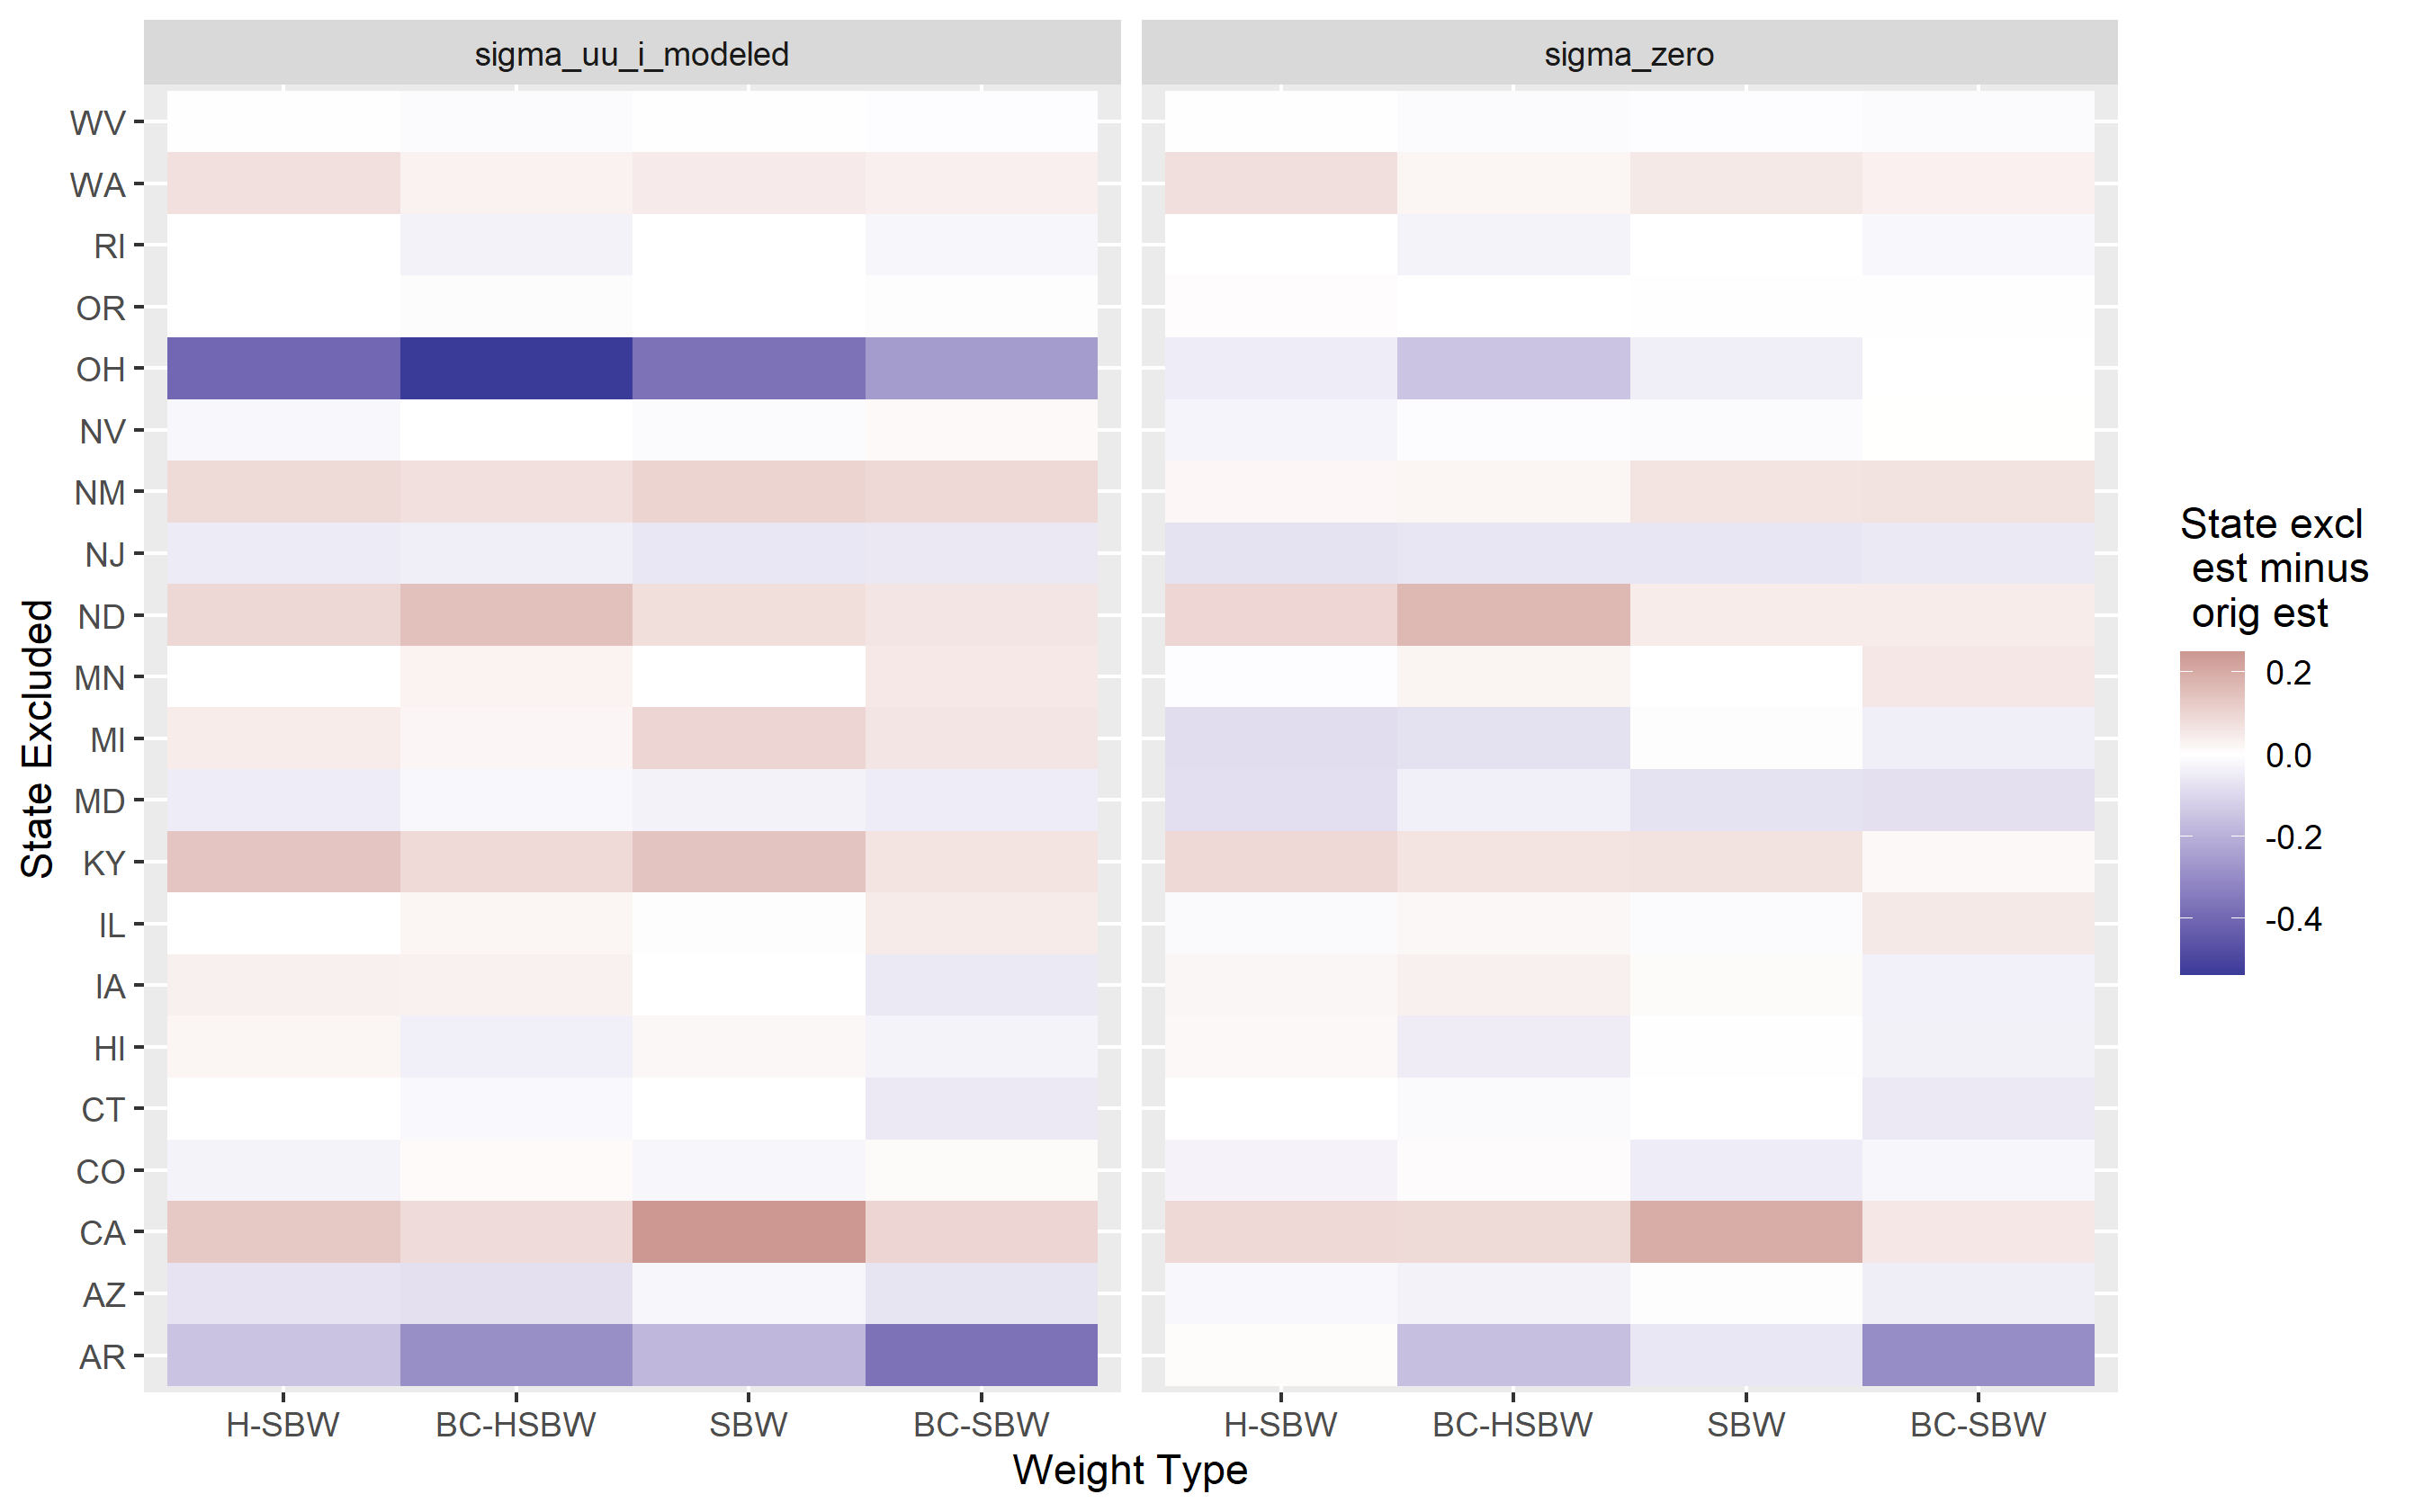
\includegraphics[scale=0.6]{01_Plots/loostate-sensitivityc1-state-uu-i.png}
\end{center}
\end{figure}

\subsection{Covariate importance}

We also investigate our hypothesis that factors associated with Governance are associated with treatment response. As discussed above, we first remove the balance constraints on the Republican governance indicators and estimate $\hat{\psi}^1_v$, and then subtract our original ETC point estimate from this quantity to generate $\hat{\Delta}_v^1$. Because this quantity does not reflect a clear population target, instead of confidence intervals, we present the minimum and maximum leave-one-state-out values in parentheses next to the original estimate.

For the H-SBW estimator we calculate $\hat{\Delta}^1$ equal to -0.69 (min = -0.83, max = -0.42) and equal to -0.79 (min = -0.90, max = -0.66) on our unadjusted dataset. In other words, our primary estimated treatment effect moved 0.78 percentage points further away from zero when we excluded the Republican governance indicators. This reflects a 33 percent decrease in our point estimate, a not-unsubstantial difference. Moreover, all of these estimates were less than zero, regardless of whether we conditioned on the covariate adjustment or not, regardless of whether we remove the early expansion states or not, and when removing each state. Across all specifications that we ran the minimum change we calculated was -1.34 and the maximum was -0.36. Additional distributional results across all leave-one-state-out estimates are available in Appendix E, Table~\ref{tab:rdiffc1}. Figure~\ref{fig:repub} displays our estimates of $\hat{\Delta}_v^1$ on our primary dataset and removing early expansion states (conditional on the covariate adjustment). 

We also consider four other covariate sets. We find that our estimates are most sensitive to controlling for pre-treatment outcomes and unemployment rates. This is not unexpected: all else equal, the expansion region had much lower pre-treatment uninsurance rates. If we do not control for these covariates, the comparable region will likely have lower pre-treament uninsurance rates, causing the estimated counterfactual to be closer to zero. The effect estimates were less sensitive to the removal of other covariate groups, and all point estimates are available in Appendix E, Table~\ref{tab:ptests}.

\begin{figure}[H]
\begin{center}
    \caption{Removing Republican Governance Indicators}
    \label{fig:repub}
    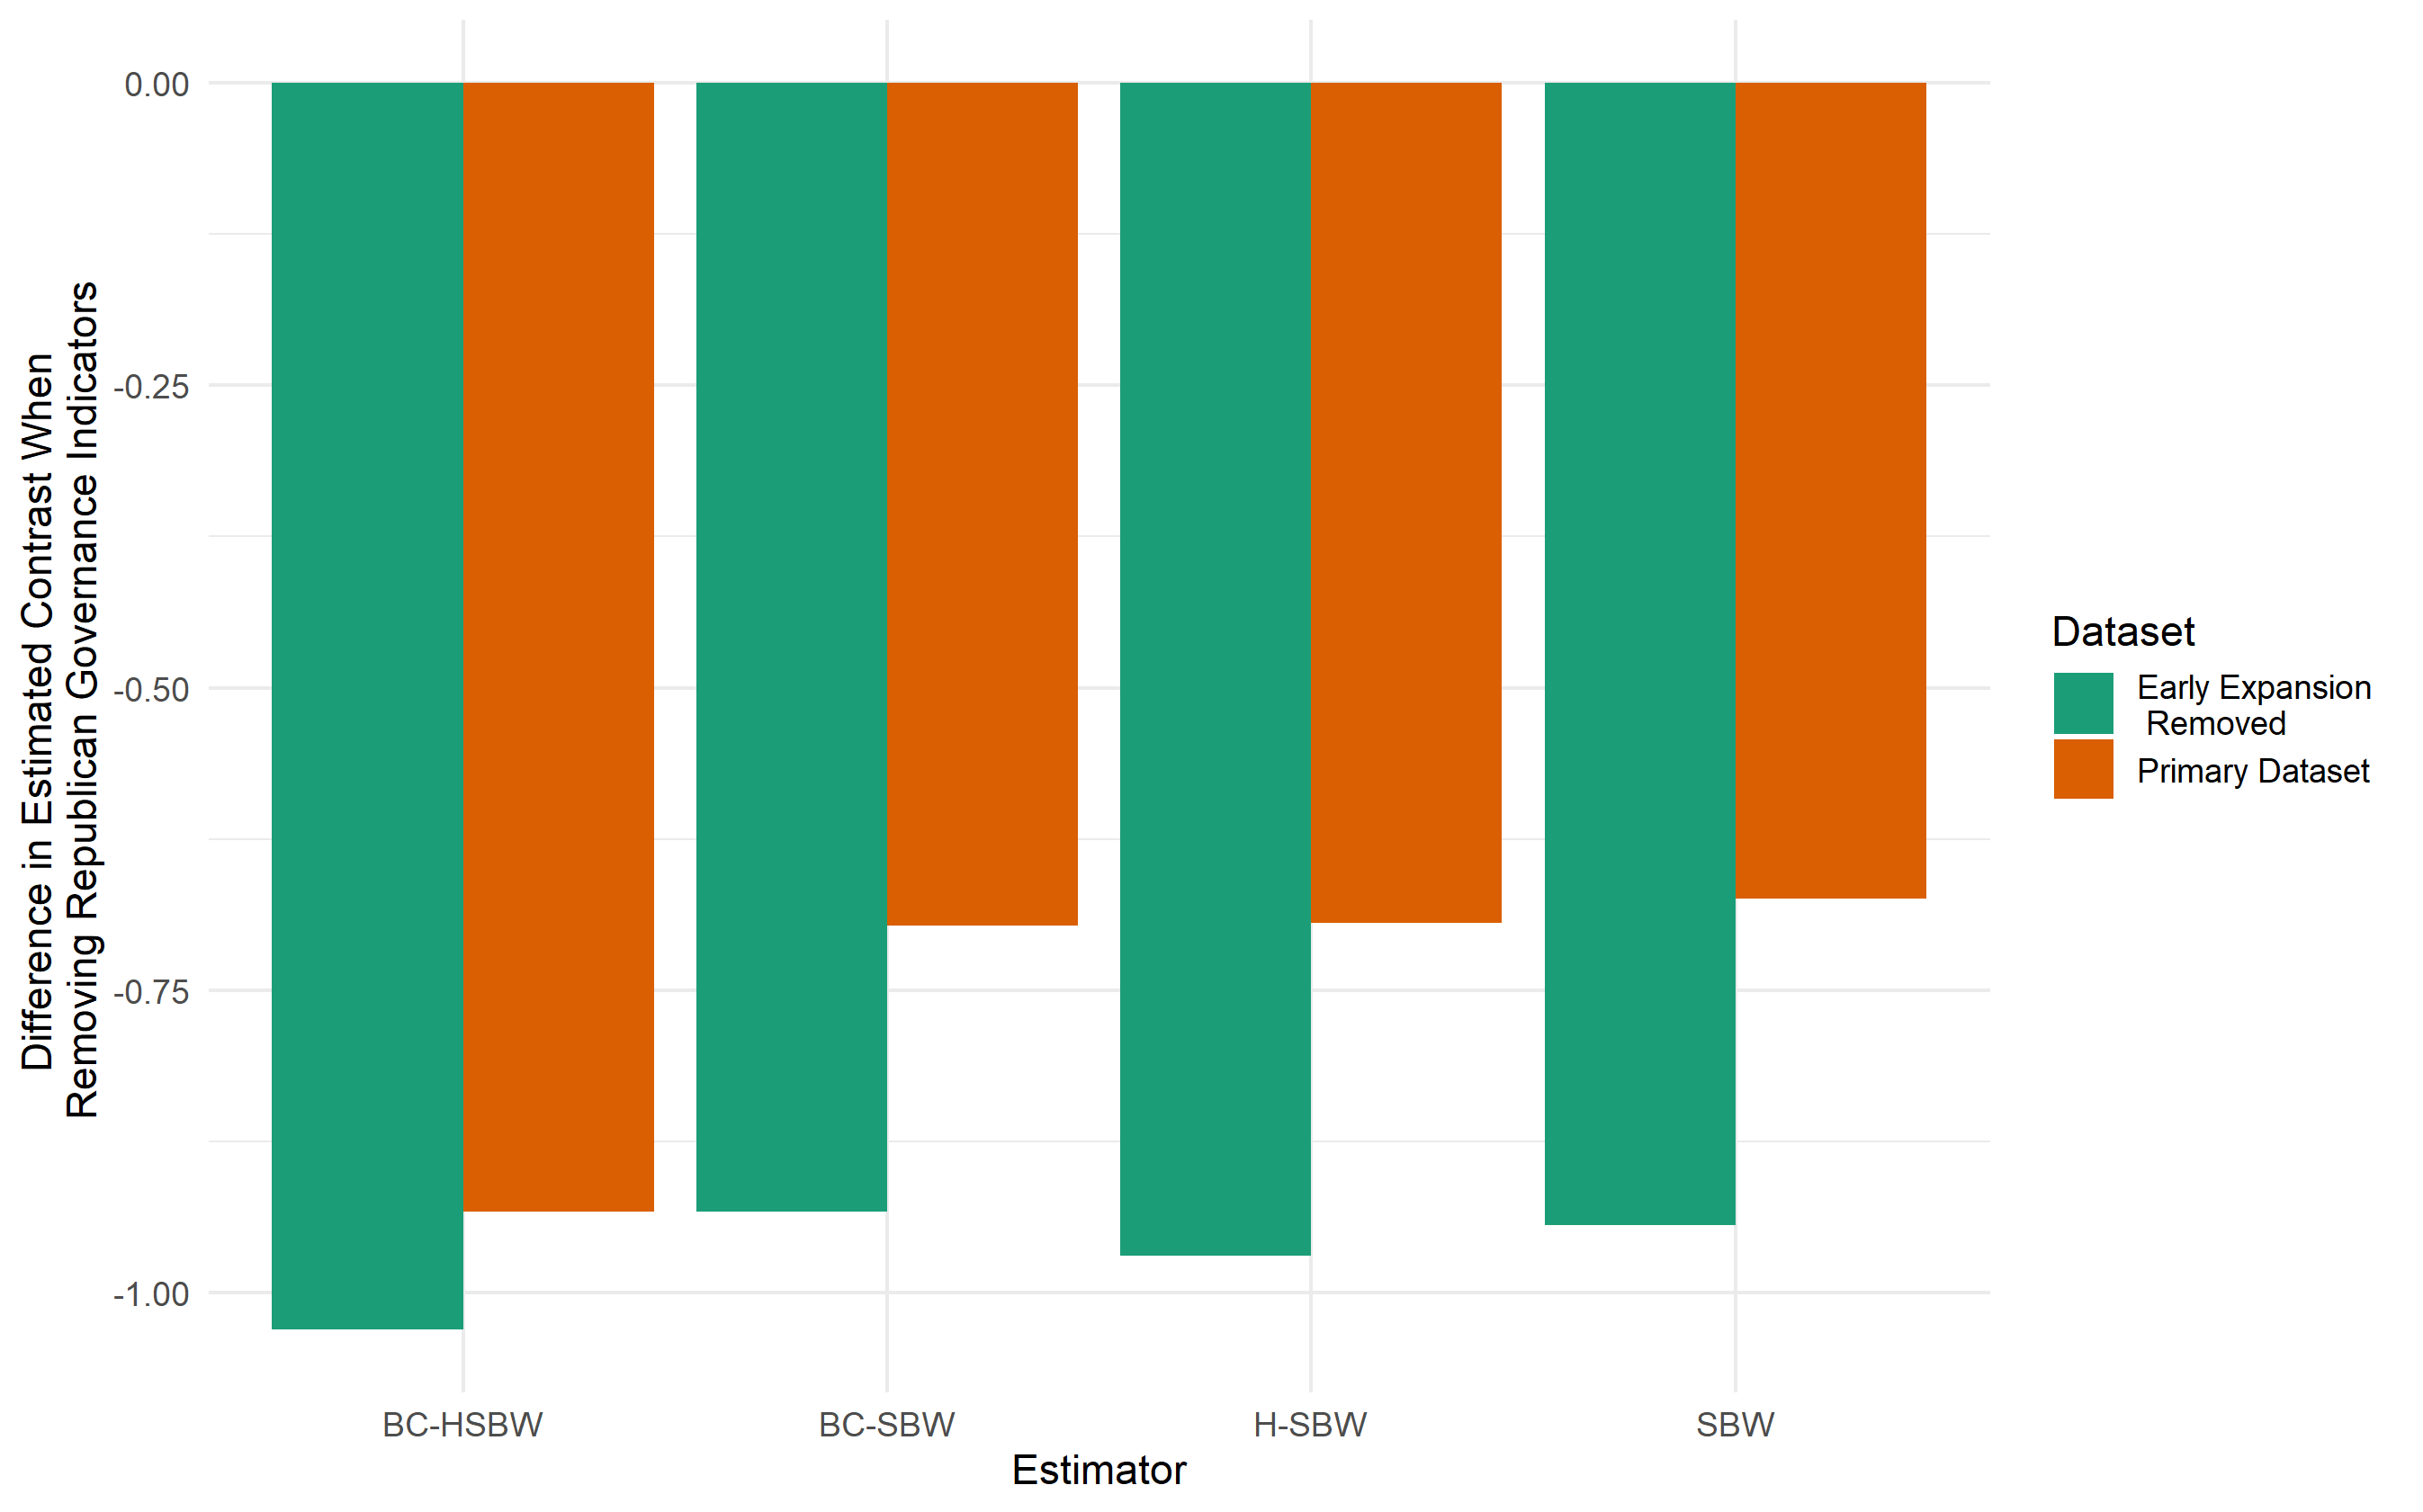
\includegraphics[scale=0.6]{01_Plots/repub-diff-all-estimators.png}
\end{center}
\end{figure}

These results highlight the importance of Republican governance in our counterfactual outcome model of $Y^1$. If the models specified by \cite{kaestner2017effects} and \cite{courtemanche2017early} are correct (that is, they correctly omit Republican governance from their balancing weights for estimating $\bar{Y}^0_{1, T}$), this would suggest treatment effect heterogeneity with respect to Republican governance. Moreover, because the expansion-state region is much more Democratic than the non-expansion region, this heterogeneity could potentially drive differences between the ETC and the ETT.

Since this is a policy question of some interest, we directly investigate this by estimating the outcome model on the full data with treatment assignment interacted with each covariate \footnote{For this analysis we calculate separate covariate adjustments on the untreated data. The summary statistics for this adjustment are available in Appendix D.}. We then examine how the estimated treatment effect would change if we decreased the interaction between treatment assignment and each Republican governance indicator -- Republican governor, Republican lower legislature control, and Republican total control -- by 50 percentage points (the original variables are either 0 or 100 and are measured at the state level). This linear combination of coefficients estimates how the treatment effect would change for any given collection of states against a set that is identical except for being 50 percentage points lower, on average, across the Republican governance indicators. We find that the linear combination is positive (0.21 percentage points) and statistically significant at the 5 percent level on the unadjusted dataset. In contrast to our previous results, this would indicate that the estimated treatment effect may be larger among Republican governed areas. However, this finding is not robust to any other specification that we run. Ultimately we interpret these results as providing no evidence of treatment effect heterogeneity with respect to Republican governance. The full results are available in Appendix E, Table~\ref{tab:hte}.

